% !TeX program = lualatex
% !TeX root = luaking.tex
% !TeX encoding = UTF-8
% !TeX spellcheck = cs_CZ
%=========================== Kapitola: Symetrie fyzikálních zákonů ================================
\setchaptertoc
\chapter{Symetrie fyzikálních zákonů}\label{fyz:IchapLII}
  \section{Symetrické operace}\label{fyz:IchapLIIsecI}
    Předmětem této kapitoly bude to, co můžeme nazvat \emph{symetrie fyzikálních zákonů}. O
    některých rysech symetrie fyzikálních Zákonů jsme již mluvili v souvislostí s vektorovou
    analýzou (kapitola \hyperref[vol03:fyz:IchapXVI]{\ref*{vol03:fyz:IchapXVI} Relativistická
    energie a hybnost}) a rotacemi (kapitola \hyperref[fyz:IchapXX]{\ref*{fyz:IchapXX} Rotace v
    prostoru}).

    Proč nás symetrie tak zajímá? Především proto, že symetrie přímo fascinuje lidskou mysl a každý
    má rád předměty nebo obrazce, jež jsou určitým způsobem symetrické. Je zajímavé, že v předmětech
    okolního světa příroda často projevuje určité druhy symetrie. Snad nejsymetričtější objekt, jaký
    si umíme představit, je koule a příroda jejich plná - jsou to hvězdy, planety, vodní kapky v
    mracích. Krystaly, které najdeme v horninách, vykazují množství různých druhů symetrie a jejich
    studiem se dozvídáme mnoho zajímavého o struktuře pevných látek. Dokonce i zvířata a rostlinná
    říše vykazují určitý stupeň symetrie, i když symetrie květu nebo včelí plástve není tak dokonalá
    a nemá tak základní význam jako symetrie krystalu. My se však nyní nebudeme zabývat tím, že v
    přírodě jsou \emph{předměty} často symetrické. Budeme se zabývat ještě pozoruhodnější symetrií
    Vesmíru - symetrií, která je v \emph{samotných základních zákonech}, jimž podléhají procesy
    fyzikálního světa.
    
    Položme si nejprve otázku: Co je to symetrie? jak může být fyzikální zákon „symetrický“? Problém
    definování symetrie je zajímavý a už jsme uváděli velmi dobrou Weylovu definici, která v podstatě
    říká, že předmět je symetrický, když s ním můžeme něco udělat a i potom bude vypadat stejně jako
    předtím. Například symetrická je váza, kterou můžeme zobrazit v zrcadlo nebo pootočit a bude
    vypadat stejně jako dříve. Nás bude zajímat, co můžeme udělat v experimentu s fyzikálním jevem
    nebo fyzikální situací, abychom dostali opět původní výsledek. Seznam známých operací, při nichž
    se nemění různé fyzikální jevy
    \begin{itemize}[noitemsep]
      \item  Translace v prostoru
      \item  Translace v čase
      \item  Rotace O pevný úhel
      \item  Pohyb po přímce konstantní rychlostí (Lorentzova transformace)
      \item  Inverze času
      \item  Zrcadlové zobrazení
      \item  Výměna stejných atomů nebo stejných částic
      \item  Změna kvantověmechanické fáze
      \item  Záměna hmoty antihmotou (nábojové sdružení)
    \end{itemize}

  \section{Symetrie v prostoru a čse}\label{fyz:IchapLIIsecII}
    První věc, o kterou se například můžeme pokusit, je \textbf{posunutí} (translace) jevů v
    prostoru. Provádíme-li experiment na určitém místě a stejnou aparaturu pak postavíme na jiném
    místě prostoru (nebo tam přemístíme původní aparaturu), vše, co se stalo v určitém časovém sledu
    s první aparaturou, se stane i s druhou, pokud zabezpečíme na obou místech stejné podmínky.
    Přitom musíme dbát na to, abychom dodrželi již zmíněnou podmínku, že budou umístěny i všechny ty
    prvky okolí aparatury, jež by mohly způsobit její odlišné chování. O tom, co vše je třeba
    přemístit a co ne, jsme už mluvili a nebudeme to v podrobnostech opakovat.
    
    Podobně jsme přesvědčení, že posunutí v čase neovlivní fyzikální zákony. (je třeba mít na
    zřeteli, že to, o čem mluvíme, se týká \emph{současného stavu poznání}, a bude proto dobře, když
    si náš výrok doplníte tvrzením: \emph{pokud je nám známo!}) Postavíme-li tedy nějakou aparaturu
    a spustíme ji v určitém okamžiku, např. ve čtvrtek v 10 hodin a pak postavíme stejnou aparaturu
    a spustíme ji za stejných podmínek např. o tři dny později, tyto aparatury budou vykonávat
    činnosti, které jsou stejnými funkcemi času bez ohledu na to, kdy začaly, pokud se podstatné
    vlastnosti okolí v obou případech stejně přizpůsobují času. Z hlediska této symetrie je stejnou
    událostí, zda jste si koupili akcie General Motors před třemi měsíci nebo dnes.
    
    Musíme však uvážit i zeměpisné rozdíly, neboť některé charakteristiky se mění se změnou polohy
    na Zemi. Když například v určité oblasti měříme magnetické pole a aparaturu pak přemístíme do
    jiné oblasti, nemusí pracovat přesně stejně, neboť tam bude jiné magnetické pole, ale tato
    odchylka bude způsobena zemským magnetickým polem. Kdybychom si však představili, že jsme
    přemístili aparaturu spolu se Zemí, rozdíl se v činnosti aparatury neprojeví.

    Další věcí, kterou jsme už podrobně prozkoumali, je rotace v prostoru. Otočíme-li aparaturu o
    nějaký úhel, bude pracovat nezměněně za předpokladu, že jsme spolu s aparaturou otočili vše, co
    je v této situaci podstatné. Problém symetrie při otáčení v prostoru jsme podrobně studovali v
    kapitole \hyperref[fyz:IchapXI]{\ref*{fyz:IchapXI} Vektory} a tam jsme zavedli
    \textbf{vektorovou analýzu} - matematický aparát umožňující velmi elegantní způsob popisu
    rotační symetrie.

    Na pokročilejším stupni se setkáváme s dalším druhem symetrie - se symetrií při rovnoměrném
    přímočarém pohybu. Je to vlastně pozoruhodný jev, že umístěním naší aparatury do rovnoměrně a
    přímočaře se pohybujícího vozidla (spolu se vším, co je pro práci aparatury podstatné) se
    nezmění chod aparatury. Jevy ve vozidle probíhají stejně, jako když vozidlo stálo, tj. všechny
    fyzikální zákony vypadají stejně. Už víme i to, jak se tato symetrie vyjádří matematický.
    Matematické rovnice fyzikálních zákonů se nesmí měnit při \emph{Lorentzově transformaci}. Bylo
    to vlastně studium problémů teorie relativity, které soustředilo zájem fyziků na symetrii
    fyzikálních zákonů.

    Uvedené symetrie měly geometrickou povahu, přičemž čas a prostor měly přibližně stejnou úlohu.
    Existují však i jiné druhý symetrií. Příkladem jiného druhu symetrie je symetrie vystihující
    skutečnost, že jeden atom můžeme nahradit jiným atomem stejného druhu. Jinak řečeno, existují
    \emph{stejné atomy}. Můžeme najít takové skupiny atomů, v nichž vzájemná záměna dvou libovolných
    atomů nezpůsobí žádnou změnu - atomy jsou identické. Vše, co může udělat jeden atom kyslíku
    určitého druhu, může udělat i jiný atom kyslíku stejného druhu. Můžete namítnout: „To je směšné,
    to je prostě \emph{definice} stejného druhu atomů.“

    Mohla by to být pouhá definice, ale pak bychom stále ještě nevěděli, zda vůbec existují atomy
    „stejného druhu“. Skutečností však je, že existuje ohromné množství atomů stejného druhu. Takže
    tvrzení, že nezáleží na tom, zda nahradíme jeden atom jiným atomem stejného druhu, skutečně něco
    znamená. Takzvané elementární částice, z nichž se skládají atomy, jsou také identickými
    částicemi v uvedeném smyslu - všechny elektrony jsou stejné, všechny protony jsou stejné,
    všechny kladné piony jsou stejné atd.

    Když jsme vyjmenovali tolik věcí, které můžeme dělat, aniž by se změnily fyzikální jevy, zdálo
    by se, že můžeme dělat prakticky všechno. Abychom ukázali, že to není pravda, všimněme si
    několika příkladů. Ptejme se:  \uv{Jsou fyzikální zákony symetrické vzhledem ke změně měřítka?}
    Předpokládejme, že jsme postavili určitý přístroj a také jiný přístroj, který má každou
    součástku pětkrát větší, a jsme zvědavi, zda tyto přístroje budou pracovat stejně. Ne, nebudou!
    Například vlnová délka světla emitovaného atomy sodíku nacházejícího se uvnitř jedné nádoby a
    vlnová délka světla emitovaného plynem sodíkových atomů v pětkrát větší nádobě budou stejné a
    nebudou v poměru jedna ku pěti. Poměr vlnové délky k velikosti zářiče se změní.

    Vezměme jiný příklad: každou chvíli vídáme v novinách obrázky modelů velkých katedrál ze zápalek
    - jsou to úžasná umělecká díla vytvořená obvykle penzisty, kteří mají čas a trpělivost k takové
    práci. Tato díla jsou ještě pečlivěji provedena a jsou úžasnější než skutečné katedrály. A nyní
    si představte, že tato dřevěná katedrála, by byla postavena ve skutečném měřítku katedrály.
    Jistě víme, co by se stalo; zřítila by se, protože zvětšené zápalky by nebyly dost silné. Někdo
    z vás by však mohl namítat, že v souladu se zvětšením měřítka by bylo třeba změnit i vnější
    vlivy. Máme na mysli schopnost předmětu odolávat gravitaci. Nejprve bychom tedy měli vzít model
    katedrály ze skutečných zápalek a skutečnou Zemi (v tom případě je katedrála stabilní) a pak
    vzít větší katedrálu a větší Zemi. To by však bylo ještě horší, neboť gravitace by ještě
    vzrostla!

    Dnes už víme, že závislost jevů na rozměrech je dána atomovým složením látky a kdyby se nám
    podařilo sestrojit tak malé zařízení, které by se skládalo jen z pěti atomů, nemohli bychom ho
    už libovolně zvětšovat nebo zmenšovat. Rozměr jednotlivého atomu není vůbec libovolný, je dán.

    Skutečnost, že fyzikální zákony nejsou neměnné při změně měřítka objevil Galilleo.  Uvědomil si,
    že pevnost materiálů není přesně úměrná jejich velikosti, a to, co jsme říkali v souvislosti s
    modelem katedrály, ilustroval na příkladu dvou kostí. Nakreslil obyčejnou kost psa v takovém
    rozměru, jaký je potřebný k udržení jeho váhy, a potom nakreslil takovou myšlenou kost, která by
    udržela „super psa“ deset nebo stokrát většího. Ta druhá kost byla velká a pevná a měla jiný
    poměr rozměrů než první kost. Nevíme, zda Galileo dospěl až k takovému závěru, že přírodní
    zákony musí mít určité měřítko. Víme však, že musel být ohromen tímto objevem a považoval ho za
    tak důležitý jako pohybové zákony, neboť je uveřejnil ve stejném díle nazvaném „O dvou nových
    vědách“.

    Uveďme další známý příklad nesymetrie zákonů. V soustavě rotující konstantní úhlovou rychlostí
    budou fyzikální zákony vypadat zcela jinak než v soustavě, která se neotáčí. Kdybychom provedli
    nějaký experiment a pak celé zařízení bychom umístili do kosmické lodi rotující v
    meziplanetárním prostoru konstantní úhlovou rychlostí, zařízení by pracovalo jinak. Víme totiž,
    že v takovém případě budou předměty uvnitř lodi vrhány ven, bude působit odstředivá síla,
    Coriolisova síla atd. Vždyť o tom, že Země rotuje, se můžeme přesvědčit pomocí Foucaultova
    kyvadla aniž bychom se dívali na hvězdy.

    Ještě se zmíníme o velmi zajímavé symetrii, která je zřejmě falešná, a tou je inverze času.
    Fyzikální zákony nemohou být zjevně obráceny v čase, neboť víme, že všechny jevy jsou ve velkém
    měřítku (tj. v našich běžných rozměrech) nevratné. Říká se: „Ruka píše, a když napsala,
    přemísťuje se dál.“ Pokud víme, tuto nevratnost způsobuje ohromné množství částic zúčastňujících
    se fyzikálních jevů, ale kdybychom rozlišili jednotlivé molekuly, nemohli bychom říci, zda
    mechanizmus pracuje tím nebo opačným směrem. Vysvětlíme to podrobněji. Mějme drobné zařízení, o
    němž víme, jak pracují jednotlivé atomy, protože můžeme pozorovat jejich pohyby. Sestrojme
    stejné zařízení, které se začne pohybovat tak, že počáteční rychlosti v novém zařízení budou
    rovny konečným rychlostem ve starém zařízení vzatým s opačnými znaménky. (v (začátek v novém) =
    - v (konec ve starém)). \emph{Toto zařízení bude konat stejné pohyby, ale přesně v opačném
    směru}. Jinak řečeno, kdybychom tedy nafilmovali se všemi podrobnostmi vnitřní pohyby v nějakém
    kusu materiálu a promítli ji na plátno v obráceném sledu, žádný z fyziků by nemohl říci: „To je
    proti fyzikálním zákonům, ten děj neprobíhá správně!“ Pokud nevidíme všechny podrobnosti,
    situace je zcela jiná. Vidíme-li, jak se vejce rozbilo na chodníku, rozbila se skořápka a
    vnitřek vytekl, určitě řekneme: „Tento děj je nevratný, neboť při opačném chodu filmu by se
    žloutek a bílek spojily, skořápka scelila, a to všechno by bylo absurdní!“ Hledíme-li však jen
    na jednotlivé atomy, zákony vypadají vratně. Odhalit tuto symetrii nebylo snadné, ale faktem je,
    že základní fyzikální zákony jsou na mikroskopické úrovni zcela vratné v čase!
  
  \section{Symetrie a zákony zachování}\label{fyz:IchapLIIsecIII}
    Už i na této úrovni jsou různé druhy symetrie fyzikálních zákonů velmi zajímavé, avšak později v
    kvantové mechanice uvidíme, jak jsou vzrušující. Ve výkladu jsme ještě nepokročili dost daleko,
    abych vám mohl říct, proč většina fyziků stále považuje za udivující a krásnou skutečnost, že v
    kvantové mechanice \textbf{každému z pravidel symetrie odpovídá určitý zákon zachování}.
    Existuje zcela určitá souvislost mezi zákony zachování a symetrií fyzikálních zákonů. My to nyní
    můžeme konstatovat, aniž bychom se to pokusili vysvětlit.
    
    Ukazuje se například, že zákony symetrie pro \emph{translaci v prostoru} vedou spolu s principy
    kvantové mechaniky k \emph{zachování hybností}.

    Zákony symetrie pro \emph{časovou translaci} vedou v kvantové mechanice k \emph{zachování
    energie}. Invariantnost vůči rotaci o pevný úhel v prostoru odpovídá \emph{zachování momentu
    hybnosti}. Tyto vztahy jsou skutečně velmi zajímavé a patří k těm nejkrásnějším a nejhlubším
    myšlenkám ve fyzice. V kvantové mechanice existují i takové symetrie, které nemají klasický
    analog a nemůžeme je popsat metodami klasické fyziky. Jedna z nich spočívá v následujícím:
    Představuje-li \(\Psi\) amplitudu nějakého procesu, pak druhá mocnina absolutní hodnoty \(\Psi\)
    představuje pravděpodobnost, že takový proces se uskuteční. Kdyby někdo jiný počítal ne s
    veličinou \(\Psi\), ale s veličinou \(\Psi'\), která se od \(\Psi\) liší jen ve fázi (je-li
    \(\Delta\) nějaká konstanta a \(\Psi'\) se od \(\Psi\) liší faktorem \(e^{\imath\Delta}\),
    dostal by pro druhou mocninu absolutní hodnoty \(\Psi'\)  (to je pravděpodobnost události)
    stejnou hodnotu jako pro druhou mocninu absolutní hodnoty \(\Psi\)

    \begin{equation}\label{fyz:eq709}
      ψ′=ψe^{\imathΔ};\qquad \abs{ψ′}^2=\abs{ψ}^2.
    \end{equation}

    Fyzikální zákony se tedy nezmění, posune-li se fáze vlnové funkce o libovolnou konstantu. To je
    další druh symetrie. Fyzikální zákony musí mít takovou povahu, že se na nich posun
    kvantověmechanické fáze neprojeví. Jak už jsme uvedli, v kvantové mechanice odpovídá každé
    symetrii určitý zákon zachování. Zdá se, že \emph{zákon zachování elektrického náboje} je
    zákonem zachování souvisejícím s \emph{kvantověmechanickou fází}. To je další velmi významný
    poznatek!
  
  \section{Zrcadlový obraz}\label{fyz:IchapLIIsecIV}
    Dalším problémem, kterým se budeme zabývat téměř v celém zbytku této kapitoly, je problém
    symetrie při zrcadlovém \emph{odrazu v prostoru}. Mohli bychom se zeptat: jsou fyzikální zákony
    symetrické vzhledem k odrazu? Tuto otázku bychom mohli formulovati takto: Předpokládejme, že
    jsme sestrojili nějaké zařízení, například hodiny, a ty mají mnoho koleček, ručiček, číslic i
    pružinu, tikají a pracují. Podívejme se na tyto hodiny v zrcadle. Nezajímá nás jejich
    \emph{vzhled} v zrcadle. \emph{Sestrojíme} ale jiné hodiny, které jsou navlas stejné jako
    vypadají první hodiny v zrcadle - všude tam, kde byl šroubek s pravotočivým závitem, bude nyní
    šroubek s levotočivým Závitem; kde byl znak „2“, bude nyní znak „\reflectbox{2}“; kde byla
    doleva stočená pružina, bude doprava stočená pružina. Když to všechno uskutečníme, budeme mít
    dvoje hodiny, oboje fyzikální a přitom budou v takovém vztahu jako předmět a jeho zrcadlový
    obraz, jenže nyní to budou dva skutečné, materiální předměty. Ptáme se: Začnou-li tyto hodiny
    jít za stejných podmínek, jejich pružiny budou stejně natažené, půjdou hodiny vždy jako
    zrcadlové obrazy? (Je to fyzikální, ne filozofická otázka.) Na tuto otázku nám naše fyzikální
    intuice odpovídá kladně, tyto hodiny by \emph{měly tak jít}.

    Máme podezření, že aspoň v případě těchto hodin je zrcadlení jednou ze symetrií fyzikálních
    zákonů, tedy když vše změníme z „levého“ na „pravé“ a vše ostatní necháme nezměněné, nezjistíme
    rozdíl. Na chvíli předpokládejme, že je to skutečně pravda. Je-li to pravda, bude nemožné
    rozlišit „pravé“ od „levého“ pomocí nějakého fyzikálního jevu právě tak, jako je například
    nemožné určit pomocí fyzikálního jevu absolutní rychlost. Pomocí fyzikálních experimentů by tedy
    nebylo možné absolutně určit, co je třeba rozumět „pravým“ v opaku k „levému“, neboť fyzikální
    zákony by byly symetrické.

    Svět samozřejmě nemusí být symetrický. V zeměpise například pojem „pravý“ můžeme zavést.
    Například, stojíme-li v New Orleanse a díváme se směrem k Chicagu, je Florida vpravo (stojíme-li
    nohama na zemi!). „Pravé“ a „levé“ tedy můžeme definovat pomocí zeměpisu. Je jen samozřejmé, že v
    libovolném systému nemusí mít skutečná situace tu symetrii, o níž mluvíme; jde však o to, zda
    jsou symetrické zákony. Jinak řečeno, zda by bylo\emph{proti fyzikálním zákonům}, kdyby
    existovala taková koule jako Země s „levostranným povrchem“ a s lidmi, kteří by se nám podobali,
    ale při pohledu z města New Orleans na město jako Chicago by viděli Floridu na opačné straně. To
    se vůbec nezdá být nemožné; záměna všeho levého na pravé není v rozporu s fyzikálními zákony.

    \begin{figure}[ht!] %\ref{fyz:fig0441}
      \centering
      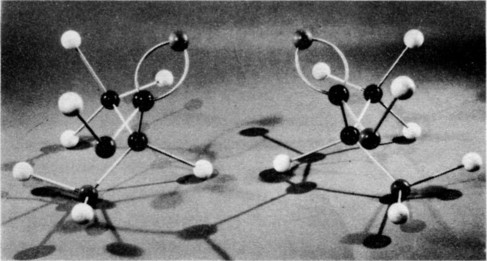
\includegraphics[width=1\linewidth]{fyz_fig0441.jpg}
      \caption{Modely alaninové molekuly.Vlevo: \emph{L}-alanin,vpravo: \emph{D}-alanin
               (\cite[s.~704]{Feynman01})}
      \label{fyz:fig0441}
    \end{figure}

    Dále musíme žádat, aby naše definice „pravého“ nezávisela na historii. Snadno bychom rozlišili
    pravé od levého, kdybychom si v železářství koupili náhodně vybraný šroubek. Tento šroubek bude
    mít pravotočivý závit - není to sice úplně jisté, ale je to velmi pravděpodobné. Příčina je v
    historii, v zavedené konvenci, ale ne v základních zákonech. Kdokoliv totiž mohl začít vyrábět
    šroubky s levotočivým závitem! 

    Musíme proto hledat takový jev, v kterém by „pravé“ vystupovalo principiálně. Další možnost, o
    níž budeme mluvit, spočívá ve skutečnosti, že polarizované světlo stáčí rovinu polarizace
    například při průchodu roztokem cukru. V kapitole
    \hyperref[fyz:IchapXXXIII]{\ref{fyz:IchapXXXIII} {Polarizace}} jsme už poznali, že rovina
    polarizace se stáčí v určitém cukrovém roztoku doprava... Tak máme způsob, jak definovat pravou
    stranu, protože nám stačí rozpustit cukr ve vodě a směr stáčení polarizační roviny nám určí
    pravou stranu. Ale cukr pochází ze živých organizmů a kdybychom ho vyrobili uměle, zjistili
    bychom, že \emph{nestáčí} rovinu polarizace! Kdybychom do uměle vyrobeného a polarizační rovinu
    nestáčejícího cukru nasadili bakterie (které se živí cukrem) a pak bakterie odfiltrovali,
    zjistili bychom, že zůstala část cukru (téměř polovina původního množství), a tento cukr stáčí
    rovinu polarizace na \emph{opačnou stranu}! I když to vypadá zamotaně, lze to snadno vysvětlit.

    Všimněme si jiného příkladu: Jednou z látek společných všem živým organizmům a nezbytných pro
    život je bílkovina. Bílkoviny se skládají z aminokyselinových řetězců. Na obrázku
    \ref{fyz:fig0441} je vidět model aminokyseliny, kterou můžeme získat z bílkoviny. Tato
    aminokyselina se nazývá alanin a její molekulární uspořádání ukazuje obr. \ref{fyz:fig0441}
    vlevo, pochází-li z bílkoviny živého organizmu. Na druhé straně, kdybychom vyrobili alanin z
    oxidu uhličitého, etanu a čpavku (a to umíme, neboť nejde o složitou molekulu), zjistili bychom,
    že vznikají stejná množství zmíněných molekul a molekul znázorněných na \ref{fyz:fig0441}
    vpravo. První molekula, ta která vzniká v živých organizmech, se nazývá \emph{L}-alanin. Druhá
    molekula, nazývaná \emph{D}-alanin, která je chemicky stejná v tom smyslu, že má stejné druhy a
    stejné vazby atomů, je „pravostrannou“ molekulou ve srovnání s „levostranným“
    \emph{L}-alaninem. Je zajímavé, že při laboratorní výrobě alaninu z jednoduchých plynů dostáváme
    ve směsi stejná množství obou druhů. Živé organizmy však používají jen \emph{L}-alanin. (Není to
    úplně pravda. Občas živé organizmy používají ke speciálním účelům i \emph{D}-alanin. Děje se to
    však velmi řídce a bílkoviny používají výlučně \emph{L}-alanin.) Vyrobíme-li oba druhy alaninu a
    touto směsí krmíme nějaké organismy, které „jedí“ nebo vychytávají alanin, spotřebují
    \emph{L}-alanin, neboť \emph{D}-alanin je pro ně nepoužitelný. Stane se tedy to, co se stalo v
    případě cukru, kdy bakterie „snědly“ jim vyhovující cukr a „špatný“ cukr nechaly! (Levotočivý
    cukr má sladkou chuť, ale jinou než pravotočivý cukr.)

    Vypadá to tak, jako by životní procesy dovolovaly rozlišit „pravé“ od „levého“, neboť takové dvě
    Molekuly jsou chemicky jiné. Jenže ve skutečnosti tomu tak není! Můžeme-li provést fyzikální
    měření takových veličin jako je energie, rychlost chemické reakce atd., dávají obě molekuly
    stejné výsledky, pokud bylo i vše ostatní zrcadlově převráceno. Jsou-li molekuly ve stejném
    množství rozpouštědla, jedny stáčejí světlo napravo a druhé stejnou mírou nalevo. Z fyzikálního
    hlediska stejně dobře vyhoví kterákoliv z těchto aminokyselin. Naše současné chápání problému je
    takové, že už v samotné Schrödingerově rovnici je zakotveno, že tyto dvě molekuly se budou
    chovat stejně až na to, že jedna se bude orientovat napravo a druhá nalevo. V životě se však
    setkáváme jen s jednou orientací.

    Předpokládá se, že příčina takové situace spočívá v následujícím. Představme si, že v určitém
    okamžiku vznikly takové podmínky pro život, že všechny bílkoviny v určitých organizmech
    obsahovaly levotočivé aminokyseliny. Když se trávicí enzymy pokoušely změnit chemické látky v
    potravě z jednoho druhu na druhý druh, jedna látka se enzymu hodila, ale druhá ne. Bylo to jako
    s Popelčiným střevíčkem, až na to, že v našem případě jde o levou nožku, na níž zkoušíme
    střevíček. Pokud víme, bylo by možné aspoň v principu vytvořit např. žábu, která by měla všechny
    molekuly převrácené. Byla by jako levostranný zrcadlový obraz skutečné žáby. Kdybychom měli
    takovou levostrannou žábu, bylo by vše v pořádku až na to, že by nenašla nic k jídlu. Kdyby
    spolkla mouchu, její enzymy by ji nemohly strávit. Moucha má totiž nevhodný druh aminokyselin
    (pokud bychom žábě nenabídli levostrannou mouchu). Vypadá to tedy tak, že kdyby bylo vše
    zrcadlově převráceno, pokračovaly by chemické a životní procesy stejným způsobem.

    Je-li život čistě fyzikální a chemický jev, pak skutečnost, že všechny bílkoviny jsou stočeny
    jedním směrem, lze pochopit jen tak, že na samém počátku náhodně zvítězil určitý druh molekul.
    Kdysi se jednou jedna organická molekula určitým způsobem zkroutila a tato událost způsobila, že
    se pravé rozrostlo v našem živém světě. Určitá historická událost byla jednostranná a od té doby
    je vše živé jednostranné. Když se dospělo do dnešního stavu, bude to už tak stále pokračovat -
    všechny enzymy tráví a produkují jen pravotočivé látky. Dostanou-li se oxid uhličitý, vodní páry
    a jiné látky do listů rostlin, enzymy produkující cukr z nich vyrobí pravostranné látky, neboť i
    tyto enzymy jsou pravostranné. Kdyby vznikl nový druh viru nebo nějaký živý organizmus, přežil
    by jen tehdy, kdyby dokázal „jíst“ ten druh živé hmoty, který už existuje. Musel by tedy být
    stejného druhu.

    Počet pravotočivých molekul se nezachovává. Tento počet může stále narůstat. Usuzujeme tedy, že
    životní jevy nemluví o tom, že by fyzikálním zákonům chyběla určitá symetrie, ale o tom, že
    všechny živé organizmy na Zemi měly společný prapůvodní počátek v uvedeném smyslu.

  \section{Polární a axiální vektory}\label{fyz:IchapLIIsecV}
    Budeme pokračovat. Ve fyzice je mnoho případů, kdy se využívají pravidla „pravé“ a „levé“ruky.
    Když jsme mluvili o vektorové analýze, uváděli jsme pravidlo pravé ruky, pomocí něhož se určuje
    správný směr momentu hybnosti, momentu síly, magnetického pole atd. Síla působící na náboj
    pohybující se v magnetickém poli je například rovna \(\vec{F} = q \vec{v}\times\vec{B}\). Není
    tato rovnice postačující k tomu, abychom v dané situaci, když známe \(\vec{F}\), \(\vec{v}\) a
    \(\vec{B}\), definovali pravou stranu? Vrátíme-li se nazpět a uvědomíme si, jak byly vektory
    zavedeny, víme, že „pravidlo pravé ruky“ bylo pouhou dohodou, jen jakýmsi trikem. Původní
    veličiny jako moment hybnosti, úhlová rychlost a ostatní podobné veličiny nebyly vůbec vektory!
    Všechny jsou nějakým způsobem spojeny s určitou rovinou a jen proto, že náš prostor je
    trojrozměrný, můžeme tyto veličiny vázat na směr kolmý k této rovině. Ze dvou možných směrů jsme
    si zvolili „pravý“.

    \begin{figure}[ht!] %\ref{fyz:fig0442}
      \centering
      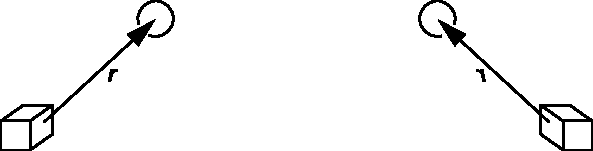
\includegraphics[width=1\linewidth]{fyz_fig0442.pdf}
      \caption{Posunutí v prostoru a jeho zrcadlový obraz (\cite[s.~706]{Feynman01})}
      \label{fyz:fig0442}
    \end{figure}

    Jsou-li fyzikální zákony symetrické, nic by se nezměnilo, kdyby se do každé fyzikální laboratoře
    vkradl jakýsi démon a v každé knize, kde vystupuje „pravidlo pravé ruky“, nahradil slovo „pravý
    “ slovem „levý“, takže by všude bylo „pravidlo levé ruky“. Ukažme to na příkladu. Existují dva
    druhy vektorů. Existují „správné“ vektory, tak jako je například posunutí \(\Delta r\) v
    prostoru. Máme-li v našem zařízení něco tady a něco jiného tam, budou tyto věci i v zrcadlovém
    zařízení, a spojíme-li původní dvě věci vektorem a podobně i zrcadlově vektorem, bude jeden
    vektor zrcadlovým obrazem druhého (obr. \ref{fyz:fig0442}). Vektor podobně jako celý prostor, se
    převrací a takový vektor nazýváme \textbf{polární vektor}.

    \begin{figure}[ht!] %\ref{fyz:fig0443}
      \centering
      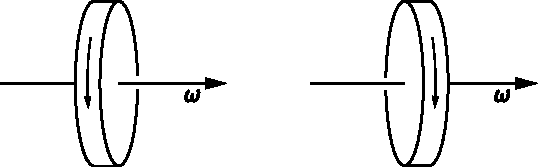
\includegraphics[width=1\linewidth]{fyz_fig0443.pdf}
      \caption{Rotující kolo a jeho zrcadlový obraz. Všimněme si že směr \uv{vektoru} úhlové 
               rychlosti se nezměnil (\cite[s.~706]{Feynman01})}
      \label{fyz:fig0443}
    \end{figure}

    S jiným druhem vektorů se setkáváme při otáčení. Představte si, že v trojrozměrném prostoru
    rotuje něco tak, jak to znázorňuje obrázek \ref{fyz:fig0443}. Na obrázku je zakreslena i rotace,
    kterou vidíme při pohledu do zrcadla; je to zrcadlový obraz původní rotace. Dohodneme se, že
    zrcadlovou rotaci popíšeme pomocí stejného pravidla jako původní rotaci; tak dostaneme „vektor“,
    který na rozdíl od polárního vektoru při odrazu nemění směr a vzhledem k polárním vektorům a
    geometrii prostoru je obrácený. Takový vektor nazýváme \textbf{axiální vektor}.

    Platí-li ve fyzice zákon symetrie při odrazu, musí být rovnice sestaveny tak, že při záměně
    znaménka každého axiálního vektoru a každého vektorového součinu, jak to odpovídá zrcadlovému
    odrazu, se nic nestane. Například, zapíšeme-li vztah pro moment hybnosti \(\vec{L} =
    \vec{r}\times \vec{p}\), bude vše v pořádku, neboť při přechodu k levé souřadnicové soustavě se
    změní znaménko \(\vec{L}\), ale \(\vec{p}\) a \(\vec{r}\) se nezmění. Znaménko vektorového
    součinu se musí změnit, musíme přejít od pravidla pravé ruky k pravidlu levé ruky. Uveďme další
    příklad. Víme, že pro sílu působící na náboj pohybující se v magnetickém poli platí vztah
    \(\vec{F} = q \vec{v}\times\vec{B}\) a vektory \(\vec{F}\) a \(\vec{v}\) jsou polární.
    Přejdeme-li od pravé soustavy k levé, musí se změna znaménka vektorového součinu kompenzovat
    změnou znaménka \(\vec{B}\), tedy \(\vec{B}\) musí být axiální vektor. Jinak řečeno při takovém
    zrcadlení musí \(\vec{B}\) přejít na \(-\vec{B}\). Změníme-li tedy souřadnice z pravých na levé,
    musíme změnit severní pól magnetu na jižní.

    \begin{figure}[ht!] %\ref{fyz:fig0444}
      \centering
      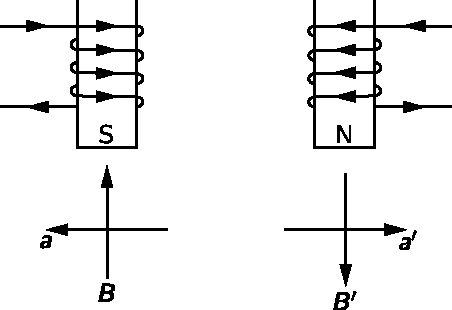
\includegraphics[width=1\linewidth]{fyz_fig0444.pdf}
      \caption{Magnet a jeho zrcadlový obraz (\cite[s.~707]{Feynman01})}
      \label{fyz:fig0444}
    \end{figure}

    Na příkladu si všimněme, jak se to stane. Mějme dva takové magnety jako na obr.
    \ref{fyz:fig0444}. První magnet má cívku navinutou určitým způsobem a teče jím proud určitým
    směrem. Druhý magnet je jako zrcadlový obraz prvního - cívku má navinutou opačně než první
    magnet a vše v ní probíhá opačně než v cívce prvního magnetu; směr proudu je zakreslen na
    obrázku. Směr magnetického pole můžeme určit ze zákonů magnetizmu, které jsme se v tomto kurzu
    ještě neučili, ale které už známe ze střední školy. Tento směr je v obou případech znázorněn na
    obrázku. V jednom případě jde o jižní magnetický pól, zatímco v druhém magnetu teče proud opačně
    a magnetické pole je obrácené - jde o severní magnetický pól. Je tedy vidět, že při přechodu od
    pravé soustavy k levé se musí změnit sever na jih!

    Záměna severu jihem ještě mnoho neříká, neboť tyto pojmy jsou dány dohodou. Musíme si proto
    všimnout samotného jevu. Předpokládejme, že v jednom poli se elektron pohybuje tak, že letí
    směrem do roviny stránky knihy. Použijeme-li vztah vyjadřující sílu, \(\vec{v} \times \vec{B}\)
    (pamatujte, že elektron nese záporný náboj), zjistíme, že ve shodě s tímto fyzikálním zákonem se
    elektron vychýlí v znázorněném směru. Jev tedy spočívá v tom, že při proudu tekoucím cívkou v
    určitém smyslu se elektron vychyluje určitým směrem. Pro fyziku není podstatné označení pólů,
    ale tento jev.

    Uskutečněme stejný experiment se zrcadlovým magnetem: poletí-li elektron uvedeným směrem, bude
    síla obrácená, pokud ji vypočítáme pomocí stejného pravidla. To je však v pořádku, neboť
    odpovídající pohyb bude zrcadlovým odrazem.

  \section{Která ruka je pravá?}\label{fyz:IchapLIIsecVI}
    Situace je taková, že při studiu jakýchkoliv jevů se setkáme s pravidlem pravé ruky dvakrát nebo
    je-li to vícekrát, je tento počet sudý. Tak se stává, že výsledný jev vypadá vždy symetricky.
    Krátce řečeno: nemůžeme-li se rozhodnout, zda jde o severní nebo jižní pól, nemůžeme rozhodnout
    ani to, zda jde o pravé nebo levé. Může se zdát, že umíme určit, který pól magnetu je severní.
    Například severní pól magnetky je ten, který směřuje na sever. jenže to je lokální vlastnost a
    máme co dělat s geografií Země; je to stejné, jako kdybychom se zeptali, kterým směrem leží
    Chicago, a to není dobrá otázka. Kdybychom si všímali magnetky, zjistili bychom, že je í severní
    konec je natřený modravou barvou. To však je už práce člověka. Jde tedy o lokální, konvenční
    kritéria.
    
    Kdyby měl magnet tu vlastnost, že při pozorném sledování by bylo na severním pólu vidět vyrůstat
    jakési chloupky, zatímco na jižním by nic takového nebylo, a to by bylo obecným pravidlem, nebo
    by existoval \emph{nějaký} jiný jednoznačný způsob rozlišení severního pólu magnetu od jižního,
    \emph{byl by to konec zákona symetrie při zrcadlení}.

    Pro lepší ilustraci celého problému si představte, že máme telefonický rozhovor s Marťanem
    nebo někým hodně vzdáleným. Přitom mu nesmíme poslat žádný vzorek k prozkoumání. Kdybychom mu
    například mohli poslat světlo, mohlo by to být světlo pravotočivě kruhově polarizované a pak by
    stačilo říci: „Všimni si, jak je světlo polarizované; takovou polarizaci nazveme pravostrannou“
    My mu však nesmíme nic poslat, smíme s ním jen mluvit a on je přitom někde velmi daleko, na
    neznámém místě a nemůže vidět nic z toho, co vidíme my. Nemůžeme mu například říct: „Podívej se
    na Velký vůz a všimni si, jak jsou rozmístěny jeho hvězdy \uv{pravou stranou rozumíme …}. My mu
    smíme jen telefonovat.

    Chtěli bychom mu o nás všechno povědět. Samozřejmě bychom začali s definováním čísel, a to tak,
    že bychom řekli: „Tik, tik - dva, tik, tik, tik - tři...“, takže by mohl postupně pochopit
    několik slov, a tak bychom pokračovali dále. Časem bychom se s ním natolik seznámili, že by se
    nás zeptal: \uv{Jak vy vlastně vypadáte?} A my bychom mu začali popisovat náš vzhled. \uv{Jsme
    \SI{175}{\cm} vysocí.} On by nás přerušil: „Moment, co to vlastně znamená - 175 centimetrů?
    “Mohli bychom mu to vysvětlit? Zcela určitě! Stačilo by říci: „Znáš průměr vodíkového atomu a
    naše výška je stejně velká jako \num{17 000 000 000} průměrů vodíkového atomu.“ Takový postup je
    možný, neboť fyzikální zákony se nezmění při změně měřítka, a tak můžeme definovat absolutní
    délku. Takovým způsobem určíme velikost našeho těla, povíme mu o tvaru našeho těla, že máme
    končetiny s pěti výrůstky na konci atd. a on pravděpodobně bez obtíží pochopí, jak navenek
    vypadáme. Dokonce si udělá podle našeho popisu model našeho těla a řekne nám: „Zvenku jste
    celkem pěkní, ale jak vypadáte zevnitř“ Pak se pustíme do popisu našich vnitřních orgánů,
    dostaneme se až k srdci, podrobně ho seznámíme s tvarem našeho srdce a řekneme mu: „Srdce máme
    na levé straně.“ Od něho dostaneme odpověď: „Hm - na levé straně?“ Bude v rozpacích, a proto mu
    musíme popsat, kde vlastně máme srdce, ale on přitom nikdy neviděl to, co vidíme my a nikdy od
    nás nedostal vzorek, podle něhož by bylo jasné, co je to pravá strana. Dokážeme to?
  
  \section{Parita se nezachovává}\label{fyz:IchapLIIsecVII}
    Ukazuje se, že zákony gravitace, elektřiny a magnetizmu i jaderných sil vyhovují principu
    zrcadlové symetrie, takže závěry z nich odvozené nám v naší úloze nepomohou. Ale v přírodě
    existuje mnoho částic, které vykazují jev nazývaný \emph{rozpad \(\beta\)} nebo \emph{slabý}
    rozpad. Jeden z případů slabého rozpadu souvisící s částicí, jež byla objevena kolem roku 1954,
    postavil před fyziky hlavolam. Vyskytla se taková nabitá částice, která se rozpadla na tři
    \(\pi\)-mezony podle schématu znázorněného na obr. \ref{fyz:fig0445}. Na určitou dobu nazvali
    tuto částici \(\varTheta\)-mezon. Na obr. \ref{fyz:fig0445b} je vidět i jiná částice, která se
    rozpadá na \emph{dva} mezony; ze zákona zachování náboje vyplývá, že jeden z nich musí být
    neutrální. Tuto částici nazvali \(\varTheta\)-mezonem. Na jedné straně tedy máme částici
    nazývanou \(\tau\), jež se rozpadá na tři \(\pi\)-mezony a na druhé částici \(\varTheta\), jež
    se rozpadá na dva \(\pi\)-mezony. Zjistilo se, že \(\tau\) a \(\varTheta\) mají téměř stejné
    hmotnosti; v rámci experimentální chyby jsou vlastně stejné. I o časech potřebných k rozpadu na
    tři \(\pi\)-mezony a na dva \(\pi\)-mezony se zjistilo, že jsou téměř zcela stejné; obě částice
    žijí stejně dlouho. Kdykoliv byly vytvořeny, vždy to bylo ve stejném poměru, řekněme
    \SI{14}{\percent} \(\tau\) ku \SI{86}{\percent} \(\varTheta\).  
  
    \begin{figure}[ht!]      %\ref{fyz:fig0445}
      \centering
      \subcaptionbox{\label{fyz:fig0445a}}{\luafigure[0.48]{fyz_fig0445a.pdf}}
      \subcaptionbox{\label{fyz:fig0445b}}{\luafigure[0.48]{fyz_fig0445b.pdf}}
      \caption{Schématický diagram rozpadu \(\tau^+\) a \(\Theta^+\) \cite[s.~708]{Feynman01}}
      \label{fyz:fig0445}
    \end{figure}

    Každý s trochou důvtipu okamžitě pochopí, že to musí být stejná částice, a ne dvě rozdílné
    částice, že vlastně vytváříme objekt, který se rozpadá dvojím způsobem. Tento objekt, který se
    může rozpadnout dvojím způsobem, má proto stejnou dobu života a stejné procentuální Zastoupení
    (jde vlastně o poměr pravděpodobností uvedených rozpadů)\footnote{Dnes této částici říkáme \(K\)
    \(mezon\) nebo \(kaon\), což je skupina čtyř mezonů, které mohou nést kvantové číslo nazvané
    „podivnost“ (angl. strangeness). V kvarkovém modelu obsahují jeden podivný kvark nebo antikvark.
    Existují \(K^+ = us\), \(K^0 = ds/sd\) a \(K^-=su\). Mají hmotnost \SI{493.667\pm0.013}{\MeV}
    (\(K^\pm\)) a \SI{497.648\pm0.022}{\MeV} (\(K^0\)). Kredit: Wikipedia}.

    V kvantové mechanice můžeme pomocí principu zrcadlově symetrie dokázat (na tomto místě
    si však nemůžeme říci jak), že je \emph{nemožné}, aby oba vzniklé produkty pocházely ze stejně
    částice - stejná částice by se \emph{nemohla} rozpadnout oběma způsoby. Zákon zachování
    odpovídající principu symetrie při zrcadlení představuje něco, co nemá klasický analog a toto
    kvantověmechanickě zachování bylo nazváno \textbf{zachování parity}. jako důsledek zachování
    parity nebo přesněji ze symetrie kvantověmechanických rovnic slabých rozpadů vůči zrcadlení by
    vyplynulo, že jedna a táž částice se nemůže rozpadnout oběma způsoby. Muselo by tedy jít o
    jakousi shodu hmotností, dob života apod. Čím víc však byl tento problém zkoumán, tím byla shoda
    pozoruhodnější a nastalo podezření, že zákon symetrie přírody vůči zrcadlení nemusí platit.

    Podezření na neplatnost tohoto zákona vedlo dva fyziky Leeho a Yanga k návrhu jiných experimentů
    s příbuznými rozpady, aby se ověřila platnost zákona i na jiných případech. První takový
    experiment provedla slečna Wu z Kolumbijskě university následujícím způsobem. Velmi silným
    magnetem při velmi nízkých teplotách působila na určitý izotop kobaltu, který se rozpadá za
    emise elektronů. Je magnetický a při dostatečně nízké teplotě tepelně pohyby příliš nerozkmitají
    atomové magnetické momenty, takže ty se uspořádají podél magnetického pole. Proto budou všechny
    atomy kobaltu tímto silným polem uspořádány rovnoběžně. Pak se rozpadnou, vyzáří elektron a
    zjistilo se, že v případě atomů uspořádaných polem, jehož vektor \(\vec{B}\) směřuje nahoru,
    bude většina emitovaných elektronů letět dolů.

    Ten, kdo není dost vnímavým pozorovatelem, nebude této poznámce připisovat velký význam, ale
    ten, kdo má smysl pro tajemství přírody, bude považovat tuto poznámku za dramatický objev.
    Vložíme-li atomy kobaltu do velmi silného magnetického pole, poletí více elektronů, které
    vznikly při rozpadu dolů a měně nahoru. Kdybychom provedli „zrcadlový“ experiment, v němž jsou
    atomy kobaltu seřazeny opačně, emitované elektrony by letěly převážně nahoru, a ne dolů; je to
    tedy \emph{nesymetrický} děj. Nyní bychom už mohli obrazně říci, že \emph{magnetu narostly ty
    chloupky}, které jsme na něm předtím marně hledali. Jižním pólem magnetu je ten pól, od něhož se
    elektrony vzniklé při \(\beta\)-rozpadu vzdalují. Tak můžeme fyzikálním způsobem odlišit severní
    pól magnetu od jižního pólu.

    Pak následovalo mnoho jiných experimentů: rozpad \(\pi\)-mezonu na \(\mu\) a \(\nu\); rozpad
    \(\mu\)-mezonu na elektron a dvě neutrina, rozpad \(\Lambda\)-částice na proton a \(\pi\)-mezon,
    rozpad \(\Sigma\)-částic a mnoho dalších rozpadů. Téměř ve všech předpokládaných případech se
    potvrdila \emph{neplatnost} principu zrcadlové symetrie. Zákon zrcadlově symetrie je tedy na
    této úrovni fyziky principiálně nesprávný.

    Stručně řečeno, nyní už můžeme Marťanovi oznámit, na které straně máme srdce. Můžeme
    mu dát následující návod: „Sestroj magnet, cívkou pusť proud, vezmi kobalt a sniž teplotu.
    Experimentální zařízení orientuj tak, aby elektrony letěly od nohou k hlavě a pak směr, jímž
    prochází proud cívkou, je směr zleva doprava.“ Pomocí takového experimentu už můžeme definovat
    pravou a levou stranu.

    Bylo předpovězeno mnoho jiných jevů. Ukázalo se, že spin, moment hybnosti kobaltového jádra,
    představuje před rozpadem pět jednotek \(\hbar\) a po rozpadu 4 jednotky. Elektron tedy odnáší
    spinový moment a úlohu přitom hraje i neutrino. Není těžké si představit, že elektron musí nést
    svůj spinový moment hybnosti orientovaný ve směru svého pohybu a podobně i neutrino. Elektron by
    se tedy měl jakoby otáčet zprava doleva, to se opravdu zjistilo. Na Kalifornském technickém
    institutu dokázali Boehm a Wapstra, že spin elektronu je orientován levotočivě. (O experimentech
    dokazujících opak se ukázalo, že jsou nesprávně!)

    Další úlohou bylo najít zákon o nezachování parity. Jaké pravidlo nám říká, kdy se parita
    nezachovává? Takové pravidlo existuje a říká, že selhání se vyskytuje jen ve velmi pomalých
    reakcích nazývaných slabé rozpady a dojde-li k narušení zachování parity, pak částice se spinem,
    jako je elektron nebo neutrino apod., vychází převážně se spinem orientovaným levotočivě. Je to
    jakési pravidlo jednostrannosti; dává do souvislosti polární vektor rychlosti a axiální vektor
    momentu hybnosti a říká, že moment hybnosti směřuje s větší pravděpodobností proti vektoru
    rychlosti než souhlasně s tímto vektorem.

    Takové je pravidlo, ale dodnes vlastně neznáme jeho příčiny. Proč platí právě toto pravidlo,
    jakou má hlavní příčinu a jak to souvisí s ostatním? Takovou nesymetrií jsme byli velmi
    překvapení a dosud jsme se z toho neprobrali, takže jsme ještě nepochopili, co znamená tato
    nesymetrie z hlediska všech ostatních pravidel. Víme však, že je to zajímavý, moderní a dosud
    nerozřešený problém, takže bude vhodné, promluvíme-li si o některých s ním souvisejících
    otázkách.

  \section{Antihmota}\label{fyz:IchapLIIsecVIII}
    Když se ztratí jedna ze symetrií, první věcí, kterou musíme udělat, je vrátit se k seznamu
    známých nebo předpokládaných symetrií a ptát se, zda některá z nich nezanikla. Ještě jsme se
    nezmínili o jedné operaci z naší tabulky, kterou nemůžeme nechat nepovšimnutou -její vztah mezi
    hmotou a antihmotou. Dirac předpověděl, že vedle elektronu musí existovat ještě jiná částice
    (nazval ji pozitron a objevil ji Anderson z Kalifornského technického institutu), která s
    elektronem úzce souvisí. Vlastnosti těchto částic jsou v určitém vztahu, splňují určitá pravidla
    korespondence: jejich energie jsou stejné, hmotnosti jsou stejné, náboje jsou opačné, ale co je
    nejdůležitější, když se tyto dvě částice setkají, anihilují se a celá jejich hmotnost přejde na
    energii, např. \(\gamma\)-záření. Pozitron nazýváme \textbf{antičásticí} elektronu a uvedené
    vlastnosti jsou pro částici a antičástici charakteristické. Z Diracovy argumentace bylo jasné,
    že i ostatní částice musí mít odpovídající antičástice. Například k protonu musí existovat
    antiproton, který označujeme symbolem \(\bar{p}\) a jenž má záporný elektrický náboj, stejnou
    hmotnost jako proton atd. Nejdůležitější vlastností však je, že proton a antiproton mohou při
    setkání anihilovat. Tuto vlastnost zdůrazňujeme, neboť lidé dost dobře nechápou, že může
    existovat neutron a antineutron a říkají: „Neutron je neutrální a jak může mít tedy antineutron
    opačný náboj?“ To, že říkáme „anti-“, neznamená, že jde právě o opačný náboj, ale jde o celý
    soubor vlastností, z nichž mnohé jsou právě opačné. Antineutron se od neutronu liší v
    následujícím. Kdybychom dali dohromady dva neutrony, zůstaly by dvěma neutrony, ale kdybychom
    dali dohromady neutron a antineutron, navzájem by anihilovaly za současného uvolnění velkého
    množství energie v podobě \(\pi\)-mezonů, \(\gamma\)-záření apod.

    Máme-li antineutrony, antiprotony a antielektrony, můžeme v principu vytvářet antiatomy.
    A to se skutečně povedlo v roce 1996 na urychlovači v CERNu, kde bylo vyrobeno 11 prvních atomů
    antivodíku. Žily jen 30 millardtin sekundy a za tu dobu uletěly \SI{10}{\m}. V roce 1997 byl
    antivodík také připraven v americkém Fermilabu. Jeden z principů symetrie ve fyzice, který
    vyplývá z rovnic, je ten, že sestrojíme-li jedny hodiny z látky a druhé z antilátky, oboje
    půjdou stejně. (Kdybychom však takové hodiny přiložili k sobě, navzájem by anihilovaly, ale to
    už je jiná záležitost.) Nyní nás může napadnout následující otázka. Z hmoty můžeme sestrojit
    dvoje hodiny-jedny „levostranné“ a druhé „pravostranné“. Můžeme například sestrojit ne obyčejné
    hodiny, ale hodiny s kobaltem a magnety a detektory elektronů, které zaznamenávají přítomnost
    elektronů vzniklých \(\beta\)-rozpadem a počítají je. Je-li zaregistrován elektron, pohne se
    sekundová ručička. Zrcadlové hodiny, které napočítají méně elektronů, půjdou jinou rychlostí.
    Zřejmě tedy můžeme sestrojit takovou dvojici hodin, v níž levostranné hodiny jdou jinak než
    pravostranné. Nyní sestrojme z hmoty hodiny, které nazveme standardní nebo pravostranné. Dále
    sestrojme z hmoty také hodiny, které nazveme levostrannými. Konstatovali jsme, že obecně
    \emph{nepůjdou} tyto hodiny stejně, ale až do tohoto významného objevu se předpokládalo, že obě
    tyto hodiny by měly jít stejně. Předpokládalo se i to, že hmota a antihmota jsou ekvivalentní,
    tedy že kdybychom sestrojili pravostranné hodiny z antihmoty stejného tvaru jako pravostranné
    hodiny z hmoty, oboje by šly stejně a totéž by platilo o levostranných hodinách z hmoty a
    antihmoty. Jinými slovy: zpočátku se předpokládalo, že \emph{všechny tyto čtvery} hodiny půjdou
    stejně. Nyní už však víme, že pravostranné a levostranné hodiny z hmoty nejsou stejné. Proto
    můžeme předpokládat, že ani pravostranné a levostranné hodiny z antihmoty nebudou stejné.

    Vzniká tedy přirozená otázka, půjdou vůbec některé hodiny stejně, a které? jinými slovy: chová
    se pravostranná hmota jako pravostranná antihmota nebo se pravostranná hmota chová jako
    levostranná antihmota? Experimenty s \(\beta\)-rozpadem, v nichž místo elektronu vystupují
    pozitrony, naznačují, „pravá“ hmota se chová jako „levá“ antihmota.

    Nakonec se tedy ukázalo, že pravolevá symetrie přece jen existuje! Kdybychom sestrojili
    levostranné hodiny ne z hmoty, ale z antihmoty, šly by stejně jako pravostranné hodiny z hmoty.
    Místo dvou nezávislých pravidel v naší tabulce symetrií by zůstalo jedno nové, kombinované
    pravidlo, mluvící o tom, že pravostranná hmota je symetrická s levostrannou antihmotou. Kdyby
    ovšem Feynman psal své přednášky o několik let později, určitě by tuto kapitolu dále rozvinul.
    Další pokusy s kaony ukázaly, že ani kombinované pravidlo s „pravostrannou hmotou“ a
    „levostrannou antihmotou“ vždy neplatí. U některých procesů je navíc třeba obrátit i znaménko
    času (CPT teorém). 

    Kdyby byl náš Marťan z antihmoty, dopadly by naše instrukce o „pravostranném“ modelu našeho těla
    opačně. Co by se stalo, kdybychom se po dlouhé konverzaci rozhodli zkonstruovat kosmické lodě a
    setkat se někde v půli cesty ve vesmíru? Určitě bychom si řekli o našich zvyklostech při
    setkávání a chtěli bychom si potřást rukama. Museli bychom se však mít na pozoru, kdyby nám náš
    kosmický přítel chtěl podat levou ruku!
  
  \section{Porušení symetrie}\label{fyz:IchapLIIsecIX}
    Je přirozené ptát se, co s takovými zákony, které jsou jen \emph{přibližně} symetrické? Co
    nejvíc udivuje, je skutečnost, že v široké oblasti důležitých jevů, jako jsou jaderné síly,
    elektrické jevy a dokonce i tak slabé interakce jako je gravitace, ve velmi rozsáhlé oblasti
    fyziky se tyto zákony ukazují být symetrické. Na druhé straně existuje jeden nepatrný jev a ten
    nám říká: „Ne, zákony nejsou symetrické!“ Jak je to možné, že příroda je téměř symetrická, ale
    přece jen symetrickou není? Co s tím máme dělat? Nejdříve si všimněme, zda neznáme nějaké jiné
    příklady tohoto druhu. Několik takových příkladů opravdu existuje. Například jaderné části sil
    mezi protonem a protonem, mezi neutronem a neutronem a mezi neutronem a protonem jsou přesně
    stejné -existuje symetrie jaderných sil, nová symetrie, která dovoluje záměnu neutronu a
    protonu. Je zřejmé, že nejde o obecnou symetrii, neboť mezi neutrony neexistuje elektrické
    odpuzování, ale existuje mezi dvěma protony. Obecně tedy neplatí, že proton můžeme nahradit
    neutronem, ale je to dobrá aproximace. Ptáte se proč \emph{dobrá}? Protože jaderné síly jsou
    mnohem silnější než elektrické. I v tomto případě jde tedy o „přibližnou“ symetrii. Vidíme, že
    existují i jiné příklady.
    
    jsme zvyklí přijímat symetrii jako projev dokonalosti. Tento náš zvyk připomíná starou představu
    Řeků o dokonalosti kruhů. V důsledku této utkvělé představy bylo přímo hrozné uvěřit, že dráhy
    planet nejsou přesně kruhové, ale jen přibližně kruhové. Rozdíl mezi kružnicí a něčím, co je
    téměř kruhové, není vůbec malý a z hlediska myšlení jde o principiální rozdíl. Kružnice nese
    znak dokonalosti a symetrie a je-li porušena, tyto momenty se ztrácejí - symetrie mizí. Samotná
    odpověď na otázku, proč jsou dráhy jen \emph{přibližně} kruhové, je příliš složitá. Skutečné
    dráhy planet jsou obecně eliptické, ale v průběhu věků pod vlivem slapových sil a podobně se
    staly téměř symetrické. Podobá se tento problém našemu problému? jde-li o kružnice, pak kdyby
    byly dokonalé, nebylo by co vysvětlovat, ale když dokonalé nejsou, je vysvětlování příliš mnoho
    a ve skutečnosti jde o složitý dynamický problém. Měli bychom vysvětlit, proč jsou dráhy planet
    přibližně symetrické z hlediska slapových sil apod.
    
    Měli bychom tedy vysvětlit, odkud symetrie pochází. Proč je příroda přibližně symetrická? To
    však dodnes nikdo neví. jediné, co můžeme navrhnout, je asi toto. V japonském městě Neiko
    existuje brána, kterou mnozí Japonci nazývají nejkrásnější v Japonsku. Byla postavena v době,
    kdy japonskou kulturu silně ovlivňovalo čínské umění.je velmi umělecky vyrobena s množstvím
    štítů, sloupů, dračích hlav, princů a nádherných rytin. Při pozorném pohledu však můžeme
    spatřit, že na jednom ze sloupů je ve složitém komplexu znaků jeden z dekoračních prvků vyrytý
    převráceně. Jinak je vše úplně symetrické. O této bráně koluje pověst, že převrácený prvek je
    tam proto, aby bohové nežárlili na dokonalost člověka. Tvůrce této brány udělal schválně chybu,
    aby zabránil hněvu bohů, který by pramenil ze žárlivosti.
    
    Proč bychom tuto myšlenku neobrátili a nepodali následující vysvětlení přibližné symetrie
    přírody? Bůh stvořil zákony jen přibližně symetrické, aby lidé nežárlili na jeho dokonalost!

%---------------------------------------------------------------------------------------------------